\documentclass[11pt]{article}
\makeatletter\def\input@path{{../}}\makeatother
\usepackage{preamble}
\usetikzlibrary{arrows.meta, positioning, fit, backgrounds}
\renewcommand{\chaptername}{Chapter 7: Case studies using hierarchical modeling}
\graphicspath{{figures/}}
% JAGS output for Chapter 7 (ch07/code/ch07_jags.R, run on GitHub Actions).
\newcommand{\JAGSsevenThree}{%
\begin{sanity}\small\textbf{JAGS output} (3 chains $\times$ 40{,}000 draws).\par\smallskip
\centering
\begin{tabular}{lcccc}\toprule
 & Mean & 95\% interval & $\hat R$ & ESS\\\midrule
$\mu_1-\mu_0$ (log OR) & $-0.846$ & $(-1.661,\ -0.097)$ & 1.001 & 16{,}520\\
$\mu_0$ (control logit) & $-2.004$ & $(-2.49,\ -1.54)$ & 1.000 & 20{,}920\\
$\mu_1$ (treatment logit) & $-2.850$ & $(-3.61,\ -2.19)$ & 1.001 & 16{,}570\\\bottomrule
\end{tabular}\par\smallskip\raggedright
$\Prob(\mu_1<\mu_0\mid\mathbf Y)=0.985$ --- the same as our sampler ($-0.850$, 0.986).
\end{sanity}}

\newcommand{\JAGSsevenFour}{%
\begin{sanity}\small\textbf{JAGS output} (3 chains $\times$ 25{,}000 draws, as the exercise asks).\par\smallskip
\centering
\begin{tabular}{lcccc|c}\toprule
 & Mean & 95\% interval & $\hat R$ & ESS & our Gibbs mean\\\midrule
$\theta_1$ & 6.182 & (6.114, 6.251) & 1.000 & 25{,}270 & 6.182\\
$\theta_2$ & 0.0387 & (0.019, 0.066) & 1.000 & 11{,}440 & 0.0385\\
$\theta_3$ & 0.990 & (0.958, 1.020) & 1.000 & 29{,}660 & 0.990\\
$\theta_4$ & 0.0087 & (0.0054, 0.0137) & 1.000 & 22{,}840 & 0.0087\\
$\theta_5$ & 2.26 & (1.49, 3.25) & 1.001 & 4{,}501 & 2.27\\
$\theta_6$ & 0.031 & (0.019, 0.047) & 1.001 & 4{,}640 & 0.031\\\bottomrule
\end{tabular}\par\smallskip\raggedright
All $\hat R\le1.001$; JAGS and our sampler agree to the third decimal.
\end{sanity}}

\newcommand{\JAGSsevenSix}{%
\begin{sanity}\small\textbf{JAGS output} (3 chains $\times$ 4{,}000 draws --- JAGS inverts a $65\times65$ matrix at every update, so only a short run is practical).\par\smallskip
\centering
\begin{tabular}{lcccc}\toprule
 & Mean & 95\% interval & $\hat R$ & ESS\\\midrule
$\mu$ & $-0.11$ & $(-3.07,\ 3.84)$ & 1.007 & 2{,}260\\
$\sigma$ & 2.12 & (0.94, 4.50) & 1.023 & 107\\
$\rho$ (km) & 79 & (8, 256) & 1.022 & 125\\\bottomrule
\end{tabular}\par\smallskip\raggedright
Consistent with our sampler (whose longer, collapsed-update chains mix better): the same wide, weakly identified range and scale.
\end{sanity}}


\tikzset{
  par/.style  = {circle, draw=navy, thick, fill=ansbg, minimum size=9mm, inner sep=1pt, font=\small},
  dat/.style  = {rectangle, draw=book, thick, fill=bookbg, minimum size=8mm, inner sep=2pt, font=\small},
  hyp/.style  = {circle, draw=idea, thick, fill=ideabg, minimum size=8mm, inner sep=1pt, font=\small},
  arr/.style  = {-{Stealth[length=2.2mm]}, thick, color=ink!80},
  plate/.style= {draw=book, rounded corners, dashed, inner sep=6pt}
}

\begin{document}

\solutionstitlepage{7}{Case studies using hierarchical modeling}{All numbers and figures are reproduced by \texttt{ch07/code/ch07.R} (hand-written samplers, base R). The JAGS versions of Exercises 3(b), 4 and 6 are in \texttt{ch07/code/ch07\_jags.R} and run on GitHub.}

\tableofcontents
\clearpage

\section*{Answers at a glance}
\addcontentsline{toc}{section}{Answers at a glance}
\begin{center}
\small
\renewcommand{\arraystretch}{1.25}
\begin{tabular}{>{\bfseries\color{navy}}r p{0.82\linewidth}}\toprule
1 & Compatible only if $a=b$ and $|a|<1$; e.g.\ $a=1,b=0.5$ is incompatible. A DAG multiplies valid conditionals in a fixed order, so the product always integrates to 1.\\
2 & DAG: $(\mu_0,\phi_0,\tau_0)\to Y_t$, $Y_{t-1}\to Y_t$, and $(Y_t,Y_{t-1},X_{j,t-1},\alpha_j,\beta_j,\phi_j,\tau_j)\to X_{jt}$.\\
3 & Pooled OR 0.53, random-effects OR 0.43 $(0.19,\ 0.90)$; both say the treatment reduces deaths; RE preferred (WAIC 73.6 vs 78.8).\\
4 & $\rho_i\approx0.99$ (near random walk); data very informative about $\theta_1$--$\theta_4$; a common-$\rho$ model is simpler and better by WAIC.\\
5 & $\lambda\mid\text{data}\sim\dist{Gamma}(a+165,\ b+69{,}593)$, $\approx0.0024$/day; men's hazard 1.65 times women's ($\Prob=0.999$).\\
6 & Range $\rho\approx66$ km (wide); maps show a high-risk eastern cluster; 10 villages have $\Prob(p_v>0.5)>0.9$.\\\bottomrule
\end{tabular}
\end{center}
\clearpage

% ================================================================= primer
\section*{A five-minute primer on the tools of this chapter}
\addcontentsline{toc}{section}{Primer: the tools of this chapter}

\begin{recall}
\textbf{1. Directed acyclic graphs (DAGs).} Each variable is a node; an arrow $A\to B$ means ``$B$'s distribution is specified given $A$''. If the graph has no directed cycles, the joint density is the product of each node's density given its parents:
\[
p(\text{all nodes})=\prod_{v}p(v\mid\text{parents}(v)).
\]
Squares will denote observed data, circles unknown parameters, and orange circles hyperparameters.

\medskip
\textbf{2. Three layers.} \emph{Data layer}: how the observations depend on the process (likelihood). \emph{Process layer}: the scientific model for the unobserved quantities. \emph{Prior layer}: distributions for the parameters.

\medskip
\textbf{3. Multivariate random effects.} $\bm\alpha_i\iid\dist N_2(\bm\mu,\bm\Sigma)$ with $\bm\Sigma\sim\dist{InvWishart}(\nu,\mathbf S)$ is conjugate: $\bm\Sigma\mid\cdot\sim\dist{InvWishart}\big(\nu+K,\ \mathbf S+\sum_i(\bm\alpha_i-\bm\mu)(\bm\alpha_i-\bm\mu)^\top\big)$.

\medskip
\textbf{4. Censored data.} An observed event at time $y$ contributes the density $f(y)$; a patient still alive at the end of follow-up $T$ contributes the survival probability $\Prob(Y>T)$.

\medskip
\textbf{5. Gaussian-process (spatial) random effects.} $\bm\alpha\sim\dist N(\mu\mathbf 1,\ \sigma^2\mathbf R(\rho))$ with $R_{uv}=e^{-d_{uv}/\rho}$: nearby locations have similar effects; $\rho$ is the \emph{range} (correlation $e^{-1}\approx0.37$ at distance $\rho$). \textbf{Elliptical slice sampling} updates the whole vector $\bm\alpha$ without tuning.
\end{recall}

\clearpage

% ================================================================= Exercise 1
\exercise{7.1 --- Can we specify a model by its full conditionals?}

\begin{problem}{1}
Since full conditional distributions are used in many MCMC algorithms, it is tempting to specify the model via its conditional distributions. For example, consider the conditional distributions:
\[
Y|X\sim\dist{Normal}(aX,1)\quad\text{and}\quad X|Y\sim\dist{Normal}(bY,1).
\]
\begin{enumerate}[(a)]
\item Select values of $a$ and $b$ so that these full conditional distributions are incompatible; i.e., there is no valid joint distribution for $X$ and $Y$ that gives these full conditional distributions. Argue, but do not formally prove, your assertion that the full conditional distributions are incompatible.
\item Explain why building a model that produces a valid DAG will always lead to a valid joint distribution.
\end{enumerate}
\end{problem}

\begin{restate}
Two conditional distributions do not always fit together into one joint distribution. Find values of $a,b$ where they do not, and explain why building a model top-down (as a DAG) avoids the problem.
\end{restate}

\begin{recall}
For a bivariate normal $(X,Y)$: $\E(Y\mid X)=\frac{\Cov(X,Y)}{\V(X)}X$ and $\V(Y\mid X)=\V(Y)-\frac{\Cov(X,Y)^2}{\V(X)}$ (and symmetrically for $X\mid Y$).
\end{recall}

\begin{keyidea}
If a joint distribution existed, it would be bivariate normal (both conditionals are normal and linear). Matching its slopes and conditional variances to $a$, $b$ and 1 gives equations that only have a solution for some $(a,b)$.
\end{keyidea}

\solution
\step{(a) Step 1 --- what a joint distribution would require.}
Let $V_X=\V(X)$, $V_Y=\V(Y)$, $C=\Cov(X,Y)$. The conditionals demand
\[
\frac C{V_X}=a,\qquad\frac C{V_Y}=b,\qquad V_Y-\frac{C^2}{V_X}=1,\qquad V_X-\frac{C^2}{V_Y}=1.
\]
\step{(a) Step 2 --- solve.} From the first two, $C=aV_X=bV_Y$. The fourth equation gives $V_X-\frac{a^2V_X^2}{aV_X/b}=V_X(1-ab)=1$, so $V_X=\frac1{1-ab}$; by symmetry $V_Y=\frac1{1-ab}$ too. Then $aV_X=bV_Y$ forces $\mathbf{a=b}$, and $V_X>0$ forces $\mathbf{ab<1}$, i.e.\ $|a|<1$.
\why{So the two conditionals are compatible only when $a=b$ with $|a|<1$ (then $X,Y$ are bivariate normal with variances $\frac{1}{1-a^2}$ and correlation $a$).}

\step{(a) Step 3 --- incompatible examples, illustrated by a Gibbs sampler.}
\begin{itemize}
\item $\mathbf{a=1,\ b=0.5}$ ($a\neq b$). A Gibbs sampler alternating the two conditionals still settles down, but to a distribution whose conditionals are \emph{not} the ones we specified: with $2\times10^5$ sweeps the output has slope 0.50 for $X$ on $Y$ but slope \textbf{0.80} for $Y$ on $X$ (we asked for 1). Theory for the sampler's limit gives exactly $b(1+a^2)/(1+b^2)=0.80$.
\item $\mathbf{a=b=2}$ ($ab>1$). Each sweep multiplies $X$ by about $ab=4$: $|X|$ is 380 after 5 sweeps, $4\times10^{5}$ after 10 and $4\times10^{17}$ after 30. No distribution can have these conditionals.
\end{itemize}

\begin{sanity}
Compatible case $a=b=0.5$: the sampler gives slopes 0.500 and 0.503 and $\V(X)=1.327$ vs.\ the theoretical $1/(1-ab)=1.333$. \checkmark
\end{sanity}

\step{(b) Why a DAG always works.} Because the graph is acyclic, the nodes can be put in an order in which every node comes after its parents. Each factor $p(v\mid\text{parents}(v))$ is a proper density in $v$. Integrating the product over the \emph{last} node removes its factor (it integrates to 1, and no other factor depends on it); repeating this for each node in reverse order shows the whole product integrates to 1 --- so it is a valid joint density, and its conditionals are exactly the specified ones. A cycle (e.g.\ $X\to Y\to X$) breaks this argument: there is no ``last'' node to integrate out first.

\begin{answer}
(a) The conditionals are compatible only if $a=b$ and $|a|<1$. For example $a=1$, $b=0.5$ (or $a=b=2$) is incompatible: matching a bivariate normal's slopes and variances is impossible, and a Gibbs sampler either converges to a distribution with different conditionals (slope 0.80, not 1) or diverges. (b) A DAG defines the joint as a product of proper conditional densities in a parents-first order; integrating out nodes from last to first shows the product integrates to 1.
\end{answer}

\begin{takeaway}
Specify models top-down (marginal, then conditionals), and let the MCMC algorithm derive the full conditionals --- not the other way round.
\end{takeaway}

% ================================================================= Exercise 2
\exercise{7.2 --- A DAG for the climate-reconstruction model}

\begin{problem}{2}
Draw a DAG for the hierarchical model in Section 7.2.3.
\end{problem}

\begin{restate}
Draw the graph of the Brisbane rainfall-reconstruction model: rainfall $Y_t$ follows an AR(1) process, and six proxy records $X_{jt}$ depend on the rainfall in the same year plus their own AR(1) errors.
\end{restate}

\begin{recall}
Section 7.2.3 model:
\begin{itemize}
\item Rainfall: $Y_1\sim\dist N(\mu_0,1/\tau_0)$, $\ Y_t\mid Y_{t-1}\sim\dist N\big(\mu_0+\phi_0(Y_{t-1}-\mu_0),\ \frac{1-\phi_0^2}{\tau_0}\big)$.
\item Proxies: $\mu_{jt}=\alpha_j+\beta_jY_t$; $\ X_{j1}\sim\dist N(\mu_{j1},1/\tau_j)$, $\ X_{jt}\mid X_{j,t-1}\sim\dist N\big(\mu_{jt}+\phi_j(X_{j,t-1}-\mu_{j,t-1}),\ \frac{1-\phi_j^2}{\tau_j}\big)$.
\item Priors on $\mu_0,\phi_0,\tau_0$ and on $\alpha_j,\beta_j,\phi_j,\tau_j$ for $j=1,\dots,6$.
\end{itemize}
\end{recall}

\begin{keyidea}
Draw one arrow into each node from every quantity that appears in its distribution. A \emph{plate} (dashed box) means ``repeat for $j=1,\dots,6$''.
\end{keyidea}

\solution
\begin{center}
\begin{tikzpicture}[node distance=14mm and 16mm]
  % rainfall layer
  \node[hyp] (mu0) {$\mu_0$};
  \node[hyp, right=of mu0] (phi0) {$\phi_0$};
  \node[hyp, right=of phi0] (tau0) {$\tau_0$};
  \node[par, below=16mm of mu0] (Ytm1) {$Y_{t-1}$};
  \node[par, right=28mm of Ytm1] (Yt) {$Y_t$};
  % proxy layer
  \node[dat, below=20mm of Ytm1] (Xtm1) {$X_{j,t-1}$};
  \node[dat, below=20mm of Yt] (Xt) {$X_{jt}$};
  \node[hyp, below=14mm of Xtm1, xshift=12mm] (ab) {$\alpha_j,\beta_j$};
  \node[hyp, below=14mm of Xt, xshift=-12mm] (pt) {$\phi_j,\tau_j$};
  % edges: rainfall
  \draw[arr] (mu0) -- (Ytm1); \draw[arr] (mu0) -- (Yt);
  \draw[arr] (phi0) -- (Yt); \draw[arr] (tau0) -- (Yt); \draw[arr] (tau0) -- (Ytm1);
  \draw[arr] (Ytm1) -- (Yt);
  % edges: proxies
  \draw[arr] (Yt) -- (Xt); \draw[arr] (Ytm1) -- (Xtm1); \draw[arr] (Ytm1) -- (Xt);
  \draw[arr] (Xtm1) -- (Xt);
  \draw[arr] (ab) -- (Xt); \draw[arr] (pt) -- (Xt);
  \draw[arr] (ab) -- (Xtm1); \draw[arr] (pt) -- (Xtm1);
  % plate
  \begin{scope}[on background layer]
    \node[plate, fit=(Xtm1) (Xt) (ab) (pt), label={[font=\footnotesize, text=book]below right:proxy $j=1,\dots,6$}] {};
  \end{scope}
\end{tikzpicture}
\end{center}
\step{Reading the graph.}
\begin{itemize}
\item \textbf{Rainfall chain}: $Y_t$ depends on the previous year's rainfall $Y_{t-1}$ and on $(\mu_0,\phi_0,\tau_0)$.
\item \textbf{Proxy chain}: $X_{jt}$ depends on this year's rainfall $Y_t$ (through $\mu_{jt}=\alpha_j+\beta_jY_t$), on last year's proxy $X_{j,t-1}$ \emph{and} last year's rainfall $Y_{t-1}$ (through $\mu_{j,t-1}$ in the AR term), and on $(\alpha_j,\beta_j,\phi_j,\tau_j)$.
\item There are no arrows from proxies to rainfall: rainfall \emph{drives} the proxies. Rainfall values $Y_t$ are partly observed (recent years) and partly missing (they become unknown nodes, imputed by MCMC); the proxies are data (squares), some also missing.
\end{itemize}

\begin{answer}
See the DAG above: $(\mu_0,\phi_0,\tau_0)\to Y_t\leftarrow Y_{t-1}$; and inside a plate over $j=1,\dots,6$: $(Y_t,\ Y_{t-1},\ X_{j,t-1},\ \alpha_j,\beta_j,\phi_j,\tau_j)\to X_{jt}$.
\end{answer}

\begin{takeaway}
Drawing the DAG first makes the code almost write itself: one JAGS line per node, with exactly the parents shown.
\end{takeaway}

% ================================================================= Exercise 3
\exercise{7.3 --- Meta-analysis of corticosteroid trials}

\begin{problem}{3}
In this problem we will conduct a meta analysis, i.e., an analysis that combines the results of several studies. The data are from the rmeta package in R:
\begin{center}
\small
\begin{tabular}{rlcccc}\toprule
 & name & ev.trt & n.trt & ev.ctrl & n.ctrl\\\midrule
1 & Auckland & 36 & 532 & 60 & 538\\
2 & Block & 1 & 69 & 5 & 61\\
3 & Doran & 4 & 81 & 11 & 63\\
4 & Gamsu & 14 & 131 & 20 & 137\\
5 & Morrison & 3 & 67 & 7 & 59\\
6 & Papageorgiou & 1 & 71 & 7 & 75\\
7 & Tauesch & 8 & 56 & 10 & 71\\\bottomrule
\end{tabular}
\end{center}
The data are from seven randomized trials that evaluate the effect of corticosteroid therapy on neonatal death. For trial $i\in\{1,\dots,7\}$ denote $Y_{i0}$ as the number of events in the $N_{i0}$ control-group patients and $Y_{i1}$ as the number of events in the $N_{i1}$ treatment-group patients.
\begin{enumerate}[(a)]
\item Fit the model $Y_{ij}|\theta_j\overset{indep}{\sim}\dist{Binomial}(N_{ij},\theta_j)$ with $\theta_0,\theta_1\sim\dist{Uniform}(0,1)$. Can we conclude that the treatment reduces the event rate?
\item Fit the model $Y_{ij}|\theta_{ij}\overset{indep}{\sim}\dist{Binomial}(N_{ij},\theta_{ij})$ with $\mathrm{logit}(\theta_{ij})=\alpha_{ij}$ and $\bm\alpha_i=(\alpha_{i0},\alpha_{i1})^T\iid\dist{Normal}(\bm\mu,\bm\Sigma)$, $\bm\mu\sim\dist{Normal}(0,10^2\mathbf I_2)$, and $\bm\Sigma\sim\dist{InvWishart}(3,\mathbf I_2)$. Summarize the evidence that the treatment reduces the death rate.
\item Discuss the advantages and disadvantages of both models.
\item Which model is preferred for these data?
\end{enumerate}
\end{problem}

\begin{restate}
Seven trials of steroids for premature babies. Combine them (a) by pooling all patients, and (b) with a random-effects model that lets each trial have its own baseline risk and treatment effect.
\end{restate}

\begin{recall}
\begin{itemize}
\item Beta--binomial (Chapter 1). Odds ratio $\text{OR}=\frac{\theta_1/(1-\theta_1)}{\theta_0/(1-\theta_0)}$; on the logit scale, the log odds ratio is $\alpha_{i1}-\alpha_{i0}$.
\item Inverse-Wishart update: primer, point 3.
\end{itemize}
\end{recall}

\begin{keyidea}
Model (a) treats all control patients as one big group and all treated patients as another. Model (b) compares treatment with control \emph{within} each trial and lets trials differ; the overall effect is $\mu_1-\mu_0$.
\end{keyidea}

\solution
\step{(a) Pooled model.} Totals: control $120/1004$, treatment $67/1007$. Posteriors $\theta_0\sim\dist{Beta}(121,\ 885)$ (mean 0.120) and $\theta_1\sim\dist{Beta}(68,\ 941)$ (mean 0.067).
\[
\Prob(\theta_1<\theta_0\mid\mathbf Y)=0.99997,\qquad\text{OR: median }0.53,\ 95\%\text{ CI }(0.39,\ 0.72).
\]
Under this model the evidence is overwhelming: the death rate is roughly halved.

\step{(b) Random-effects model --- sampler.} Each iteration: (i) a Metropolis step for all seven $\bm\alpha_i$ at once (acceptance 47\%), using the binomial likelihood and the $\dist N_2(\bm\mu,\bm\Sigma)$ prior; (ii) $\bm\mu\mid\cdot\sim\dist N_2\big(\mathbf V\bm\Sigma^{-1}\sum_i\bm\alpha_i,\ \mathbf V\big)$ with $\mathbf V=(7\bm\Sigma^{-1}+\mathbf I/100)^{-1}$; (iii) $\bm\Sigma\mid\cdot\sim\dist{InvWishart}\big(10,\ \mathbf I+\sum_i(\bm\alpha_i-\bm\mu)(\bm\alpha_i-\bm\mu)^\top\big)$. Three chains $\times$ 35{,}000 kept draws; $\hat R=1.000$ and ESS $=11{,}227$ for $\mu_1-\mu_0$.
\step{(b) Results.}
\[
\mu_1-\mu_0:\ \text{mean }-0.85,\ 95\%\text{ CI }(-1.67,\ -0.11),\qquad\Prob(\mu_1<\mu_0\mid\mathbf Y)=0.986,\qquad\text{OR median }0.43.
\]
\begin{center}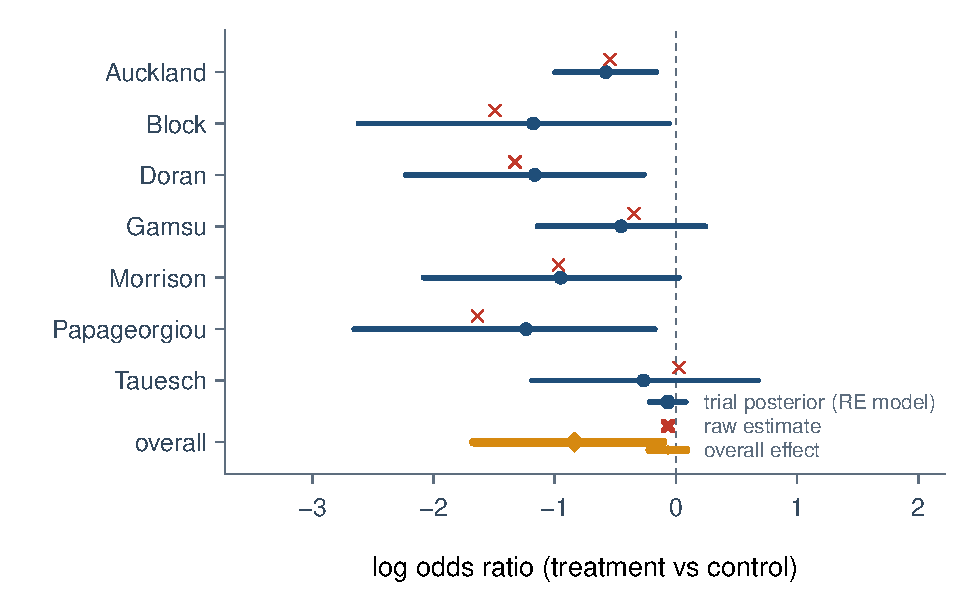
\includegraphics[width=0.78\linewidth]{ex03_forest.pdf}\end{center}
Six of seven trials individually favour treatment; the small trials (Block, Doran, Papageorgiou) are pulled toward the overall effect; Tauesch (the only trial with a positive raw log-OR) is pulled down to $-0.26$.
\JAGSsevenThree

\step{(c) Advantages and disadvantages.}
\begin{itemize}
\item \textbf{Pooled model} --- \emph{pros}: simple, two parameters, precise. \emph{Cons}: ignores that trials differ (baseline mortality ranges from 8\% to 18\% across control arms), so it can be biased if treatment/control ratios differ between trials (Simpson's paradox), and its interval is too narrow; it also discards the randomisation \emph{within} trials.
\item \textbf{Random-effects model} --- \emph{pros}: compares arms within each trial (respecting randomisation), allows between-trial heterogeneity in both baseline risk and effect, gives trial-specific shrunken estimates. \emph{Cons}: more complex, needs MCMC, results depend on the prior for $\bm\Sigma$ (only 7 trials to estimate a $2\times2$ covariance), and the overall effect is less precise.
\end{itemize}

\step{(d) Which is preferred?} WAIC (over the 14 trial-arm counts): pooled 78.8, random effects \textbf{73.6}. The random-effects model fits clearly better, and it is the scientifically appropriate design for a meta-analysis.

\begin{answer}
(a) Yes under the pooled model: $\Prob(\theta_1<\theta_0)\approx1$, OR 0.53 (0.39--0.72). (b) The random-effects model also supports a benefit: log-OR $-0.85$ $(-1.67,-0.11)$, $\Prob(\text{reduction})=0.986$, OR $\approx0.43$, with a wider interval. (c) Pooled: simple but ignores heterogeneity and within-trial randomisation; RE: realistic but more complex and prior-sensitive. (d) The random-effects model (WAIC 73.6 vs.\ 78.8).
\end{answer}

\begin{takeaway}
Meta-analyses should compare arms \emph{within} studies. Pooling raw counts across studies can mislead when studies differ in size and baseline risk.
\end{takeaway}

% ================================================================= Exercise 4
\exercise{7.4 --- A hierarchical model for marathon pacing}

\begin{problem}{4}
Download the marathon data of Section 6.4 from the course webpage. Let $Y_{ij}$ be the speed of runner $i$ in mile $j$. Fit the hierarchical model $Y_{i1}\sim\dist{Normal}(\mu_i,\sigma_0^2)$ and
\[
Y_{ij}|Y_{ij-1}\sim\dist{Normal}(\mu_i+\rho_i(Y_{ij-1}-\mu_i),\sigma_i^2),
\]
where $\mu_i\iid\dist{Normal}(\theta_1,\theta_2)$, $\rho_i\iid\dist{Normal}(\theta_3,\theta_4)$, and $\sigma_i^2\iid\dist{InvGamma}(\theta_5,\theta_6)$.
\begin{enumerate}[(a)]
\item Draw a DAG for this model, and give an interpretation for each parameter in the model.
\item Select uninformative prior distributions for $\theta_1,\dots,\theta_6$.
\item Fit the model in JAGS using three chains each with 25,000 iterations, and thoroughly assess MCMC convergence for the $\theta_j$.
\item Are the data informative about the $\theta_j$? That is, are the posterior distributions more concentrated than the prior distributions?
\item In light of (c) and (d), are there any simplifications you might consider, and if so, how would you compare the full and simplified models?
\end{enumerate}
\end{problem}

\begin{restate}
Each runner has a typical pace $\mu_i$, a ``stickiness'' $\rho_i$ (how much last mile's deviation carries over) and a mile-to-mile variability $\sigma_i^2$; these vary across runners according to hyperparameters $\theta_1,\dots,\theta_6$.
\end{restate}

\begin{recall}
\begin{itemize}
\item Data: 2016 Boston Marathon, top female runners, pace in minutes per mile for miles 1--26 (book website). We use the 58 runners with no missing splits (as in Section 2.1.7).
\item Given $\rho_i$, the mean structure is linear in $\mu_i$: $Y_{ij}-\rho_iY_{i,j-1}=(1-\rho_i)\mu_i+\varepsilon_{ij}$. Given $\mu_i$, it is a regression through the origin of $e_{ij}=Y_{ij}-\mu_i$ on $e_{i,j-1}$ with slope $\rho_i$. So almost everything is conjugate.
\end{itemize}
\end{recall}

\begin{keyidea}
Gibbs sampling for $\mu_i$, $\rho_i$ (normal), $\sigma_i^2$, $\sigma_0^2$ (inverse-gamma), $\theta_1,\theta_3$ (normal), $\theta_2,\theta_4$ (inverse-gamma), $\theta_6$ (gamma); a Metropolis step for the shape $\theta_5$.
\end{keyidea}

\solution
\step{(a) DAG.}
\begin{center}
\begin{tikzpicture}[node distance=12mm and 13mm]
  \node[hyp] (t12) {$\theta_1,\theta_2$};
  \node[hyp, right=of t12] (t34) {$\theta_3,\theta_4$};
  \node[hyp, right=of t34] (t56) {$\theta_5,\theta_6$};
  \node[par, below=of t12] (mu) {$\mu_i$};
  \node[par, below=of t34] (rho) {$\rho_i$};
  \node[par, below=of t56] (s2) {$\sigma_i^2$};
  \node[dat, below=16mm of mu] (Y1) {$Y_{i1}$};
  \node[dat, right=10mm of Y1] (Yjm1) {$Y_{i,j-1}$};
  \node[dat, right=14mm of Yjm1] (Yj) {$Y_{ij}$};
  \node[hyp, left=10mm of Y1] (s0) {$\sigma_0^2$};
  \draw[arr] (t12) -- (mu); \draw[arr] (t34) -- (rho); \draw[arr] (t56) -- (s2);
  \draw[arr] (mu) -- (Y1); \draw[arr] (s0) -- (Y1);
  \draw[arr] (mu) -- (Yj); \draw[arr] (rho) -- (Yj); \draw[arr] (s2) -- (Yj); \draw[arr] (Yjm1) -- (Yj);
  \begin{scope}[on background layer]
    \node[plate, fit=(mu) (rho) (s2) (Y1) (Yjm1) (Yj), label={[font=\footnotesize, text=book]below right:runner $i=1,\dots,58$; mile $j=2,\dots,26$}] {};
  \end{scope}
\end{tikzpicture}
\end{center}
\step{(a) Interpretation.}
\begin{itemize}
\item $\mu_i$: runner $i$'s long-run average pace (min/mile); $\rho_i$: persistence --- the fraction of a fast/slow deviation that carries into the next mile ($\rho_i\approx1$: the runner drifts; $\rho_i\approx0$: each mile bounces back to $\mu_i$); $\sigma_i^2$: runner $i$'s mile-to-mile variability; $\sigma_0^2$: variability of the first mile around $\mu_i$.
\item $\theta_1,\theta_2$: mean and variance of the typical pace across runners; $\theta_3,\theta_4$: mean and variance of persistence across runners; $\theta_5,\theta_6$: shape and scale of the distribution of the runners' variabilities.
\end{itemize}

\step{(b) Uninformative priors.} $\theta_1\sim\dist N(0,100^2)$, $\theta_3\sim\dist N(0,10^2)$ (both far wider than plausible values), $\theta_2,\theta_4\sim\dist{InvGamma}(0.1,0.1)$, $\theta_5,\theta_6\sim\dist{Gamma}(0.1,0.1)$, $\sigma_0^2\sim\dist{InvGamma}(0.1,0.1)$.

\step{(c) Convergence} (our Gibbs sampler: three chains from very different starting hyperparameters, 25{,}000 iterations each, 5{,}000 burn-in):
\begin{center}
\small
\begin{tabular}{lccccc}\toprule
 & Mean & SD & 95\% interval & $\hat R$ & ESS (of 60{,}000)\\\midrule
$\theta_1$ (mean pace) & 6.182 & 0.035 & (6.114, 6.251) & 1.000 & 19{,}253\\
$\theta_2$ (var.\ of pace) & 0.039 & 0.012 & (0.019, 0.066) & 1.000 & 11{,}979\\
$\theta_3$ (mean $\rho$) & 0.990 & 0.016 & (0.958, 1.020) & 1.000 & 22{,}118\\
$\theta_4$ (var.\ of $\rho$) & 0.0087 & 0.0021 & (0.0055, 0.0137) & 1.000 & 24{,}769\\
$\theta_5$ (shape) & 2.27 & 0.45 & (1.49, 3.27) & 1.001 & 1{,}534\\
$\theta_6$ (scale) & 0.031 & 0.007 & (0.019, 0.048) & 1.001 & 1{,}720\\
$\sigma_0$ & 0.177 & 0.029 & (0.126, 0.239) & 1.000 & 9{,}981\\\bottomrule
\end{tabular}
\end{center}
\begin{center}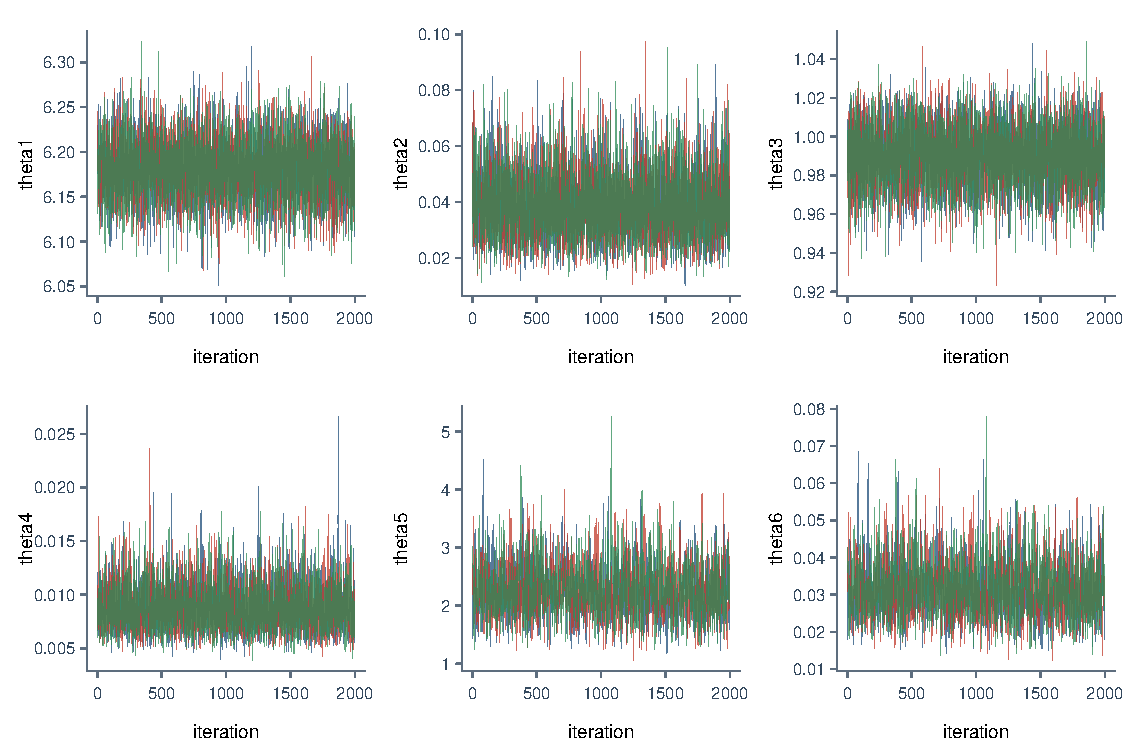
\includegraphics[width=0.98\linewidth]{ex04_traces.pdf}\end{center}
All $\hat R\le1.001$, overlapping trace plots from dispersed starts; $\theta_5,\theta_6$ mix most slowly (they are strongly correlated: shape and scale trade off), but their ESS still exceeds 1{,}500.
\JAGSsevenFour

\step{(d) Are the data informative?} Yes, very. $\theta_1$: prior SD 100 $\to$ posterior SD 0.035; $\theta_3$: prior SD 10 $\to$ 0.016. The inverse-gamma/gamma priors for $\theta_2,\theta_4,\theta_5,\theta_6$ have enormous (or infinite) spread, while the posteriors have 95\% widths of 0.046, 0.008, 1.8 and 0.029. The least informed are $\theta_5,\theta_6$ (the distribution of 58 variances), which is also why they mix slowest.

\begin{center}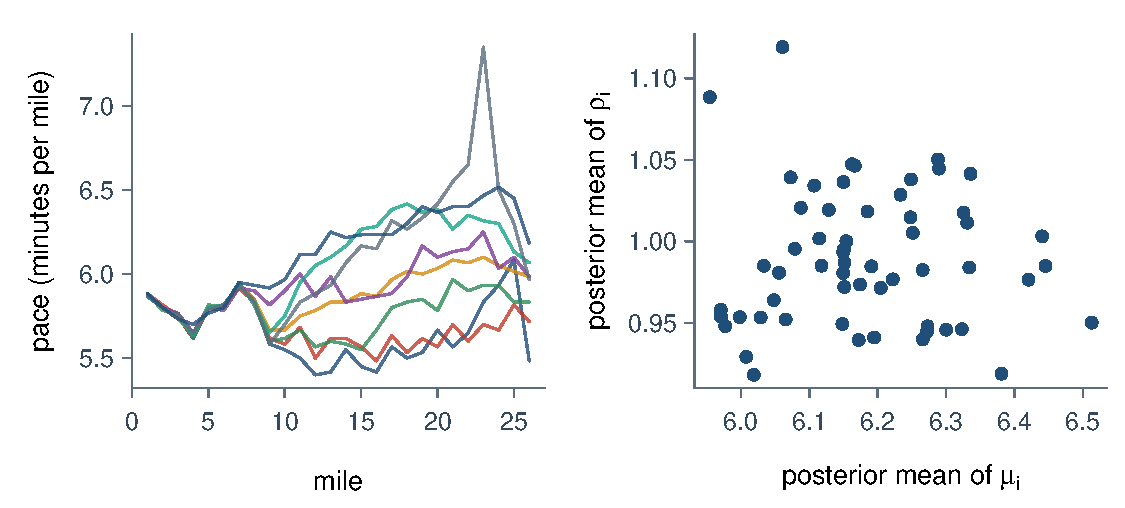
\includegraphics[width=0.98\linewidth]{ex04_runners.pdf}\end{center}

\step{(e) Simplifications and how to compare.}
The posterior of $\theta_3$ is $\approx0.99$ and $\theta_4$ is tiny (between-runner SD of $\rho_i$ about 0.09): every runner's pace behaves almost like a random walk with similar persistence. Natural simplifications:
\begin{enumerate}[(i)]
\item a \textbf{common} $\rho$ for all runners ($\theta_4=0$);
\item a random walk ($\rho_i=1$), i.e.\ model the mile-to-mile \emph{changes};
\item a common $\sigma^2$.
\end{enumerate}
Compare with WAIC (or LOO-CV) computed from the same one-step-ahead likelihood. For (i): common $\rho=1.018$ (1.004--1.031) and
\begin{center}
\begin{tabular}{lccc}\toprule
Model & lppd & $p_W$ & WAIC\\\midrule
full (runner-specific $\rho_i$) & 963.3 & 148.9 & $-1628.8$\\
common $\rho$ & 930.8 & 91.6 & $\mathbf{-1678.3}$\\\bottomrule
\end{tabular}
\end{center}
The common-$\rho$ model fits almost as well with 57 fewer effective parameters and has the lower WAIC: the simplification is supported. ($\rho$ slightly above 1 means deviations slowly \emph{grow}: runners who slow down tend to keep slowing.)

\begin{answer}
(a) DAG above; $\mu_i$ = typical pace, $\rho_i$ = persistence, $\sigma_i^2$ = variability, $\theta$'s = their population mean/variance (and shape/scale). (b) Vague normal priors for $\theta_1,\theta_3$; vague inverse-gamma/gamma for the rest. (c) Converged ($\hat R\le1.001$, ESS $\ge1{,}500$); JAGS agrees. (d) Yes: posteriors are far more concentrated than the priors, least so for $\theta_5,\theta_6$. (e) A common persistence $\rho$ (or a random walk) is a sensible simplification; by WAIC it is better ($-1678$ vs.\ $-1629$).
\end{answer}

\begin{takeaway}
When a hierarchical variance ($\theta_4$) is estimated to be small, consider removing that level: it simplifies the model and often improves prediction.
\end{takeaway}

% ================================================================= Exercise 5
\exercise{7.5 --- Exponential survival with censoring: the lung data}

\begin{problem}{5}
Download the lung data from the survival package in R. Let $Y_i$ be the survival time (days) for subject $i\in\{1,\dots,n\}$. We will make the unrealistic assumption that the survival times follow an exponential distribution, $Y_i|\lambda\sim\dist{Exponential}(\lambda)$. The study runs from time 0 to time $T$, with patient $i$ joining the study at time $T-T_i$ so that they are part of the study for $T_i$ days. The analysis is complicated by censoring; i.e., some patients have not experienced their event at the conclusion of the study. An event is observed if $Y_i<T_i$ and censored if $Y_i>T_i$, with $\delta_i=I(Y_i>T_i)$ denoting the binary indicator that the event is censored. For uncensored patients with $\delta_i=0$, the contribution to the likelihood function is the exponential PDF, $\lambda\exp(-\lambda y_i)$; for censored patients with $\delta_i=1$, the contribution to the likelihood function is the probability that they survive beyond $T_i$ days, $\exp(-\lambda T_i)$.
\begin{enumerate}[(a)]
\item Write the likelihood function in terms of the parameter $\lambda$ and the data $(Y_1,T_1,\delta_1),\dots,(Y_n,T_n,\delta_n)$.
\item Derive a conjugate prior distribution for $\lambda$, and propose hyperparameters that lead to an uninformative prior distribution.
\item Using the full dataset, summarize the posterior distribution of $\lambda$ under a few conjugate priors (i.e., different hyperparameters). Are the results sensitive to the prior?
\item Using an uninformative conjugate prior, analyze the data separately for men and women, and test whether the survival distribution varies by sex.
\end{enumerate}
\end{problem}

\begin{restate}
Estimate the death rate of 228 advanced lung-cancer patients, many of whom were still alive at the end of follow-up, and compare men and women.
\end{restate}

\begin{recall}
Censoring: primer, point 4 (and Exercise 2.12). In R's \texttt{lung} data, \texttt{time} is the observed follow-up $t_i=\min(Y_i,T_i)$ and \texttt{status} is 2 for a death, 1 for censored.
\end{recall}

\begin{keyidea}
The likelihood depends only on the number of deaths $d=\sum_i(1-\delta_i)$ and the total time at risk $\sum_it_i$; it is a Gamma kernel in $\lambda$.
\end{keyidea}

\solution
\step{(a) Likelihood.}
\[
L(\lambda)=\prod_{i=1}^n\big[\lambda e^{-\lambda Y_i}\big]^{1-\delta_i}\big[e^{-\lambda T_i}\big]^{\delta_i}
=\lambda^{\sum_i(1-\delta_i)}\exp\Big\{-\lambda\sum_i\big[(1-\delta_i)Y_i+\delta_iT_i\big]\Big\}=\lambda^{d}e^{-\lambda\sum_it_i}.
\]
\step{(b) Conjugate prior.} $L(\lambda)$ has the form $\lambda^{\text{power}}e^{-\lambda\times\text{constant}}$, so a $\dist{Gamma}(a,b)$ prior is conjugate:
\[
p(\lambda\mid\text{data})\propto\lambda^d e^{-\lambda\sum t_i}\cdot\lambda^{a-1}e^{-b\lambda}\ \Rightarrow\ \lambda\mid\text{data}\sim\dist{Gamma}\Big(a+d,\ b+\sum_it_i\Big).
\]
Uninformative: small $a$ and $b$, e.g.\ $a=b=0.01$ (worth 0.01 deaths in 0.01 days of follow-up).
\step{(c) Full data} ($n=228$, $d=165$ deaths, 63 censored, $\sum t_i=69{,}593$ days):
\begin{center}
\small
\begin{tabular}{lcccc}\toprule
Prior & Posterior & Mean rate/day & median survival & 95\% interval\\\midrule
$\dist{Gamma}(0.01,0.01)$ & $\dist{Gamma}(165.01,\ 69{,}593)$ & 0.00237 & 292 days & (0.00202, 0.00275)\\
$\dist{Gamma}(0.1,0.1)$ & $\dist{Gamma}(165.1,\ 69{,}593)$ & 0.00237 & 292 days & (0.00202, 0.00275)\\
$\dist{Gamma}(1,1)$ & $\dist{Gamma}(166,\ 69{,}594)$ & 0.00239 & 291 days & (0.00204, 0.00276)\\
$\dist{Gamma}(10,1000)$ & $\dist{Gamma}(175,\ 70{,}593)$ & 0.00248 & 280 days & (0.00213, 0.00286)\\\bottomrule
\end{tabular}
\end{center}
(Median survival $=\log2/\lambda$.) Not sensitive: vague priors are indistinguishable, and even the informative $\dist{Gamma}(10,1000)$ prior (worth 10 deaths in 1{,}000 days, mean 0.01/day) moves the rate by only 4\%.

\step{(d) Men vs.\ women.}
Men: 112 deaths in 39{,}086 days; women: 53 deaths in 30{,}507 days. With $\dist{Gamma}(0.01,0.01)$ priors:
\[
\lambda_{\text{men}}\approx0.00287,\quad\lambda_{\text{women}}\approx0.00174\text{ per day};\qquad
\Prob(\lambda_{\text{men}}>\lambda_{\text{women}}\mid\text{data})=0.999,
\]
hazard ratio men/women: median 1.65, 95\% CI (1.20, 2.31).
\begin{center}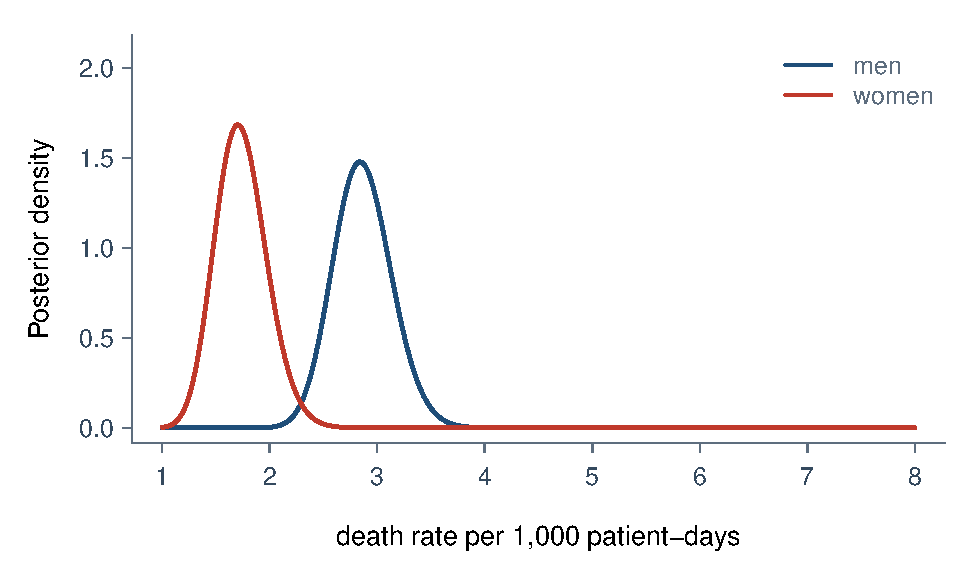
\includegraphics[width=0.68\linewidth]{ex05_sex.pdf}\end{center}
A Bayes factor for ``separate rates'' vs.\ ``common rate'' (closed form, Gamma$(a,b)$ prior on each rate):
\begin{center}
\begin{tabular}{lcc}\toprule
Prior on each rate & prior mean rate & BF(separate : common)\\\midrule
$\dist{Gamma}(1,\ 0.001)$ (absurdly vague) & 1000 per day & 0.0001\\
$\dist{Gamma}(1,\ 100)$ & 0.01 per day & 8.0\\
$\dist{Gamma}(1,\ 420)$ (centred on the pooled rate) & 0.0024 per day & 16.4\\
$\dist{Gamma}(2,\ 840)$ & 0.0024 per day & 22.4\\\bottomrule
\end{tabular}
\end{center}
With any \emph{sensible} prior the BF is 8--22 (substantial to strong evidence for different rates); a ridiculously vague prior reverses it (Lindley's paradox again).

\begin{answer}
(a) $L(\lambda)=\lambda^{d}e^{-\lambda\sum_it_i}$ with $d=\#$deaths and $t_i$ the follow-up times. (b) $\lambda\sim\dist{Gamma}(a,b)\Rightarrow\dist{Gamma}(a+d,\ b+\sum t_i)$; uninformative $a=b=0.01$. (c) $\lambda\approx0.0024$/day (median survival $\approx290$ days), insensitive to the prior. (d) Men die at about 1.65 times the rate of women (95\% CI 1.20--2.31; $\Prob=0.999$); BF 8--22 under sensible priors: survival differs by sex.
\end{answer}

\begin{takeaway}
Posterior probabilities of a direction ($\lambda_m>\lambda_f$) are robust; Bayes factors need a prior that is realistic for the scale of the problem.
\end{takeaway}

% ================================================================= Exercise 6
\exercise{7.6 --- A spatial model for village malaria prevalence}

\begin{problem}{6}
Download the Gambia data
\begin{lstlisting}
> library(geoR)
> data(gambia)
> ?gambia
\end{lstlisting}
The data consist of 2,035 children that live in 65 villages. For village $v\in\{1,\dots,65\}$, denote $n_v$ as the number of children in the sample, $Y_v$ as the number of children that tested positive for malaria, and $p_v$ as the true probability of testing positive for malaria. We use the spatial model $\alpha_v=\mathrm{logit}(p_v)$, where $\bm\alpha=(\alpha_1,\dots,\alpha_{65})^T$ follows a multivariate normal distribution with mean $\E(\alpha_v)=\mu$, variance $\V(\alpha_v)=\sigma^2$ and correlation $\Cor(\alpha_u,\alpha_v)=\exp(-d_{uv}/\rho)$, where $d_{uv}$ is the distance between villages $u$ and $v$. For priors assume $\mu\sim\dist{Normal}(0,10^2)$, $\sigma^2\sim\dist{InvGamma}(0.1,0.1)$, and $\rho\sim\dist{Uniform}(0,d^*)$ where $d^*$ is the maximum distance between villages.
\begin{enumerate}[(a)]
\item Specify the data layer, process layer and prior layer for this hierarchical model.
\item Fit the model using JAGS and assess convergence.
\item Summarize the data and results using five maps: the sample size $n_v$, the sample proportion $Y_v/n_v$, the posterior means of the $p_v$, the posterior standard deviations of the $p_v$, and the posterior probabilities that $p_v$ exceeds 0.5.
\end{enumerate}
\end{problem}

\begin{restate}
Model each village's malaria prevalence so that nearby villages tend to be similar, and map the results.
\end{restate}

\begin{recall}
Gaussian-process random effects and elliptical slice sampling: primer, point 5.
\end{recall}

\begin{keyidea}
The village logits $\bm\alpha$ are a spatially correlated random field. Collapsing $\sigma^2$ out of the update for the range $\rho$ greatly improves mixing (the two are strongly dependent).
\end{keyidea}

\solution
\step{(a) The three layers.}
\begin{itemize}
\item \textbf{Data layer}: $Y_v\mid p_v\overset{indep}{\sim}\dist{Binomial}(n_v,p_v)$, $v=1,\dots,65$.
\item \textbf{Process layer}: $\alpha_v=\mathrm{logit}(p_v)$, $\ \bm\alpha\sim\dist N\big(\mu\mathbf 1,\ \sigma^2\mathbf R(\rho)\big)$, $R_{uv}=\exp(-d_{uv}/\rho)$.
\item \textbf{Prior layer}: $\mu\sim\dist N(0,10^2)$, $\sigma^2\sim\dist{InvGamma}(0.1,0.1)$, $\rho\sim\dist{Uniform}(0,d^*)$ with $d^*=273$ km.
\end{itemize}
\step{(b) Fitting.} Our sampler, per iteration: elliptical slice sampling for $\bm\alpha$; $\mu\mid\cdot$ normal; $\rho$ by Metropolis on $\mathrm{logit}(\rho/d^*)$ with $\sigma^2$ integrated out; then $\sigma^2\mid\cdot$ inverse-gamma. Three chains (started at $\rho=5,40,120$ km) $\times$ 20{,}000 kept draws.
\begin{center}
\begin{tabular}{lccccc}\toprule
 & Mean & SD & 95\% interval & $\hat R$ & ESS (of 60{,}000)\\\midrule
$\mu$ & $-0.15$ & 1.45 & $(-2.81,\ 3.54)$ & 1.001 & 7{,}297\\
$\sigma$ & 2.00 & 1.00 & (0.93, 4.46) & 1.002 & 705\\
$\rho$ (km) & 66 & 69 & (8, 252) & 1.006 & 430\\\bottomrule
\end{tabular}
\end{center}
\why{$\rho$ and $\sigma$ are weakly identified from 65 villages (a long range with a large variance looks much like a short range with a smaller variance), so their posteriors are wide and they mix slowest. The collapsed $\rho$ update raised their ESS from about 65--90 to 430--700.}
Village probabilities $p_v$: $\hat R$ between 1.000 and 1.046, ESS 70--several thousand (median 186). This is adequate for posterior means and probabilities in the maps, though a longer run would tighten the Monte Carlo error for a few villages with no positive children.
\JAGSsevenSix

\step{(c) Five maps} (plus the posterior of $\rho$):
\begin{center}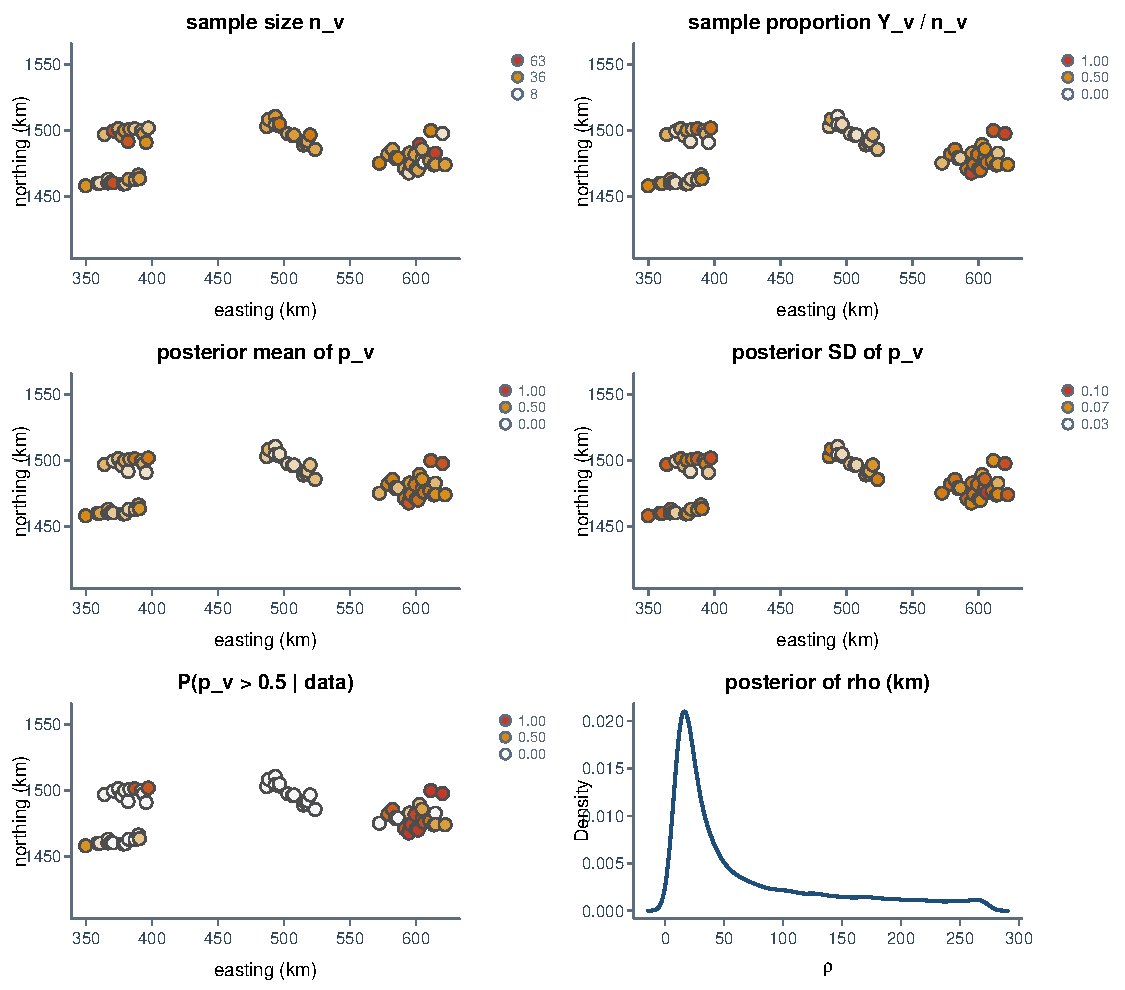
\includegraphics[width=0.98\linewidth]{ex06_maps.pdf}\end{center}
\begin{itemize}
\item \textbf{Sample sizes} range from 8 to 63 children per village.
\item \textbf{Sample proportions} are noisy, from 0 to 0.93; the eastern cluster has the highest rates.
\item \textbf{Posterior means} are smoothed versions of the sample proportions (correlation 0.98): villages with few children are pulled toward their neighbours.
\item \textbf{Posterior SDs} are largest for small villages and for villages whose rate differs from their neighbours'.
\item \textbf{$\Prob(p_v>0.5\mid\text{data})$}: 10 villages exceed 0.9 --- all of them in the eastern cluster (easting 595--620 km) --- natural targets for intervention.
\end{itemize}

\begin{answer}
(a) Data: $Y_v\sim\dist{Bin}(n_v,p_v)$; process: $\mathrm{logit}(\mathbf p)\sim\dist N(\mu\mathbf1,\sigma^2e^{-\mathbf D/\rho})$; priors as given. (b) Converged ($\hat R\le1.006$ for $\mu,\sigma,\rho$; JAGS agrees); $\sigma\approx2.0$, range $\rho\approx66$ km but very uncertain (8--252 km). (c) The maps show a high-prevalence eastern region; 10 villages have $\Prob(p_v>0.5)>0.9$.
\end{answer}

\begin{takeaway}
Spatial models turn noisy village-level counts into a smooth risk map with honest uncertainty --- exactly what is needed to target malaria control.
\end{takeaway}

\end{document}
